\documentclass[10pt,a4paper]{article}

\usepackage{times}
\usepackage{url}
\usepackage{graphicx}

\pagestyle{empty}

\textheight=25cm
\textwidth=15cm
\topmargin=-2cm
\oddsidemargin=0cm

\begin{document}

\begin{center}
  Dr Ole Nielsen \\
  Australia-Indonesia Facility for Disaster Reduction, AusAID Jakarta \\
  P: +62 811 820 4637,\ \ \ E: Ole.Moller.Nielsen@gmail.com
\end{center}
\begin{center}
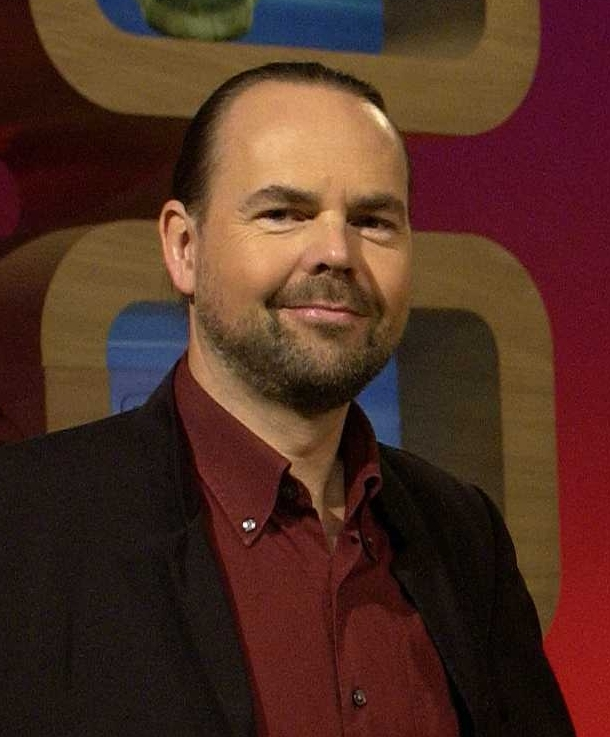
\includegraphics[width=40mm,keepaspectratio=true]{ole.jpg}
\end{center}


\begin{center}
  \hrulefill \\
  {\bf Expression of Interest: Development Manager, ICTIS, Geoscience Australia} \\[-0.2cm]
  \hrulefill
\end{center}

This is to express my sincere interest in the new position as Development Manager at ICTIS.
I was pleased to read this role description and to see that core values such as \emph{software quality}, \emph{good development practices} and \emph{coherence of development teams} have been elevated and formalised within Geoscience Australia.
%Software quality measures such as \emph{regression testing}, \emph{standards compliance}, \emph{issue tracking}, \emph{continuous integration}, \emph{priorisation linked to requirements}, \emph{error reporting} and \emph{revision control} are critical to the succes of any software engineering activity and something I have always adhered to in my work. Moreover, quality web services and interoperable delivery of data are fundamental ways for an organisation like GA to remain relevant to its stakeholders.
Since I joined Geoscience Australia in 2003 my work has revolved around what the Development Manager role embodies. In particular, experience with life-cycles, standards and best practices is evidenced by my track record of leading successful projects as is my experience in mentoring both professional contractors and junior graduates.\\

\noindent \textbf{The ANUGA hydrodynamic modelling project} which is a sophisticated open source software model written in Python and C, that has underpinned all tsunami inundation modelling in Australia. Under my leadership, this project lead to two AGM team awards: 2006 (Capability) and 2007 (Influence); was featured in 2009 in a special episode on the Australian TV program The New Inventors \emph{Dealing With Disasters} and attracted the Emergency Management Australia "Safer Communities Award" in 2005 and 2007 as well as the "Asia-Pacific Spatial Excellence Award" in 2007. ANUGA was developed as a strongly test driven project (now with almost 1,000 unit tests) and a comprehensive regression test suite of physical validation examples. ANUGA was released as Open Source in December 2006 (the first from GA) and has since then had over 16,000 downloads and is now used widely outside the organisation - e.g.\ for urban flood modelling.\\

\noindent \textbf{InaSAFE} a novel and user friendly open source application for rapid and reproducible estimation of impact from natural disasters developed by AusAID. Version 1.0 was officially launched at the Asian Ministerial Conference on Disaster Risk Reduction in October 2012 and shown to the president of Indonesia as the centrepiece of Australian Indonesian cooperation in Disaster Management. InaSAFE is currently being provided to local and national disaster managers in Indonesia.
I lead the development in a changing, distributed and demanding environment with a team of approximately 6 developers located in Indonesia, South Africa, Switzerland and Washington DC. Strong adherence to testing has been crucial to keep this project focused and a Jenkins server is continually monitoring the test suite, code coverage, adherence to PEP8 coding standards and pylint quality measures. We also have tests for multilingual support, license status of bundled data and correctness of generated graphics. We are using github for revision control, project management and issue tracking. As part of this work, I influenced the developers of a new web application geospatial interoperability, called \mbox{GeoNode}, with much needed recognition of continuous integration and regression testing and also key developers of the Quantum GIS project to elevate the importance of testing and adherence to coding styles for increased software quality.\\

\noindent \textbf{Influence on software development} which I argue has contributed to the creation of this very position:
   When I joined the organisation, there was a perception that \emph{GA does not engage in software development} and clearly very little corporate visibility of these activities. When inquiring to the EB I discovered that real position was that \emph{GA should not rely on ``hero codes'' for mission critical systems}. In 2005 I revived and chaired the Programmer's User Group (PUG) to address this very issue and put forward the proposal that \emph{the EB and developers may be able to agree that GA needs a corporate apprach ot software development}. PUG rapidly grew to over 100 members and conducted a software development survey across the organisation which revealed that more than 10\% of GA staff saw themselves as developers. This survey was taken to the executive board who noted the importance of software development and the need for good development practices (21 March 2006).
         %I handed PUG over to Stephen Lloyd on 1 June 2007 after reflecting on the achievements of the group: Established forum for software development in GA with participation of over 10\% staff, the EB resolutions, a dozen projects under revision control (managed voluntarily by Michael Moore), software discoverability initiative (Peter Petkovic) and QA/QC template being discussed (Varjavandi/Zhang).

I Dec 2006 I gave a DGAL presentation in which I demonstrated the crucial requirement for software quality assurance and showed the way forward for GA in regard to testing and validation of complex software projects.
At the 2008 AGM I won the individual award for capability based on my corporate work. The text opens with
\begin{quote}
  \emph{“Truly outstanding” is the best way to sum up the leadership that Ole has shown in the use of high performance computing and professional software engineering to support a wide range of applications within Geoscience Australia}
\end{quote}
and the award closes with
\begin{quote}
  \emph{In particular, Ole’s discipline and demand for high quality software engineering has allowed the tsunami risk modelling team to undertake challenging cutting-edge projects for a number of clients with confidence that our tools can meet varied requirements}.
\end{quote}
 I wrote a minute to the divisional chief thanking for the award but also noting that corporate software development still need access to appropriate development practices and tools.\\

\noindent \textbf{High performance computing} has been crucial for our modelling work over the years. Starting with a prototype Beowulf cluster in 2003, I oversaw all stages of negotiating, procuring, installing, testing of two larger clusters named ``cyclone'' (2004) and ``tornado'' (2006). Moreover, I liaised with the National Computing Infrastructure (NCI) in 2008 to carry out pilot projects from different divisions in GA to explore the feasibility of using NCI for GA's business needs.\\

\noindent \textbf{Other achievements and corporate contributions}
\begin{itemize}
    \item Participated in the tender panel for the 2007 AGIMO government wide survey of use of Open Source.
    \item Lead stress testing of faulty web application (flood studies database) and worked with the web team to trouble shoot and fix issue that only appeared when application was receiving heavy traffic.
    \item When requested acted as mediator in conflict resolution for the ATWS at a critical point in this project.
    \item Based on work at GA, I developed and deployed in 2011 a real time earthquake impact prediction system in the Indonesian Government agency for disaster management (BNPB).
    \item Together with Dr Adele Bear (GA), I developed a volcanic ash modelling application (python-FALL3D) and supported its validation through several workshops involving scientist from Indonesia, Phillipines, Italy and Australia.
    \item Together with Nick Horspool (GA) and Jonathan Griffin (AusAID), I supported earthquake and tsunami modelling with expertise in software design, high performance computing and testing.
    \item I have built and maintained all the required computational infrastructure (Beowulf Cluster, NAS server, Web server, Subversion/TRAC server) used at our program at AusAID from 2009 to present.
\end{itemize}

If I fill this role, I will enjoy focusing on the work I have been pursuing in GA for 10 years towards a vision of \emph{Geoscience Australia fulfilling its potential as an organisation with a reputation for producing software and data delivery systems of the highest quality and usability}.


\subsubsection*{References}
Dr Trevor Dhu (Current Manager, AusAID): Trevor.Dhu@ausaid.gov.au\\
Dr Jane Sexton (Colleague since 2005, GA): Jane.Sexton@ga.gov.au\\
%Dr Lesley Wyborne (Reference, GA): Lesley.Wyborne@ga.gov.au\\
Nick Horspool (Colleague, GA): Nick.Horspool@ga.gov.au\\
Dr Adele Bear (Colleague, GA): Adele.Bear@ga.gov.au\\
Jonathan Griffin (Colleague, AusAID): Jonathan.Griffin@ausaid.gov.au\\
Dr John Schneider (Former group leader, GA): John.Schneider@ga.gov.au\\
Prof Stephen Roberts (Collaborator on the ANUGA project, ANU): Stephen.Roberts@anu.edu.au\\

\subsubsection*{Sincerely}
Ole Nielsen

\end{document}

